\documentclass[twocolumn]{article}
\usepackage{graphicx}
\usepackage[utf8]{inputenc} % UTF8 input encoding
\usepackage[T1]{fontenc} % font encoding
\usepackage{amsmath, amssymb, mathtools, bm, nicefrac, mathrsfs} % matematik-pakker
\raggedbottom
\newcommand{\sub}[1]{_{\mathrm{#1}}}
% make \abs{} as I like it:
\DeclarePairedDelimiter\abs{\lvert}{\rvert}
	\DeclarePairedDelimiter\norm{\lVert}{\rVert}
	\makeatletter
	\let\oldabs\abs
	\def\abs{\@ifstar{\oldabs}{\oldabs*}}
	\let\oldnorm\norm
	\def\norm{\@ifstar{\oldnorm}{\oldnorm*}}
\makeatother

\begin{document}
\title{Exercise "latex" - Error Function (ODE representation)}
\date{}
\author{Mikkel Elkjær Pedersen}
\maketitle

\section{Error Function}
In this report we briefly describe the error function.
The error function arises in many branches of mathematics and physics. As a basic example, we first consider statistics.
The error function, erf(x), is closely related to the standard normal distribution,
as it exactly describes the probability for a standard normally distributed random variable $X$ to yield a value in the interval
$[-x,x]$, where x is a non-negative number. Thus the error function is a heavily studied function in mathematics.\\

In figure \ref{fig:erf} the ODE-representation of the error function is shown. Recalling the standard normal distribution, that is the Gaussian with
mean $0$ and variance $0.5$, it is clear that the error function is just the derivative of the Gaussian. This is just another way of stating
the statistical remark above. Thus $\mathrm{erf}(0)=0$ is a natural initial condition when calculating the ODE-representation by numerically integrating.
One may also implement the property of the error function that it is an odd function, that is $\mathrm{erf}(-x) = - \mathrm{erf}(x)$ for any real $x$.
This is of course a direct consequence of the Gaussian with mean $0$ being even. When numerically integrating it is of great importance to
provide a small enough step around $x=0$ to get a proper ODE-representation - for $x$'es farther from $0$ the step size can be increased
quite a lot as the function is very flat for $\abs{x} > 3$.\\

As a last remark we give an example of how to produce the error function with an experiment. A typical laser beam has a Gaussian intensity distribution
perpendicularly to the propagation direction of the light. Thus if one measures the intensity of the laser beam perpendicularly to its propagation 
- e.g. with a photodiode -, one may use the "knife edge method" to characterize the laser beam. That is, one carefully blocks an increasingly
larger part of the beam by inserting a straight sharp object in between the laser and the photo diode. 
If one registers the beam intensity as a function of how far the knife has "cut" through the laser beam one should produce exactly the error function
assuming the laser beam is Gaussian. One may then carry out this method in two mutually perpendicular directions, both of whom are perpendicular
to the beam propagation, to acchieve a 2D profile of the laser beam. Thus it can be examined if for instance the waist of the beam are of equal
size horizontally as vertically or if the beam profile is in fact Gaussian at all.

\begin{figure}
% GNUPLOT: LaTeX picture with Postscript
\begingroup
  \makeatletter
  \providecommand\color[2][]{%
    \GenericError{(gnuplot) \space\space\space\@spaces}{%
      Package color not loaded in conjunction with
      terminal option `colourtext'%
    }{See the gnuplot documentation for explanation.%
    }{Either use 'blacktext' in gnuplot or load the package
      color.sty in LaTeX.}%
    \renewcommand\color[2][]{}%
  }%
  \providecommand\includegraphics[2][]{%
    \GenericError{(gnuplot) \space\space\space\@spaces}{%
      Package graphicx or graphics not loaded%
    }{See the gnuplot documentation for explanation.%
    }{The gnuplot epslatex terminal needs graphicx.sty or graphics.sty.}%
    \renewcommand\includegraphics[2][]{}%
  }%
  \providecommand\rotatebox[2]{#2}%
  \@ifundefined{ifGPcolor}{%
    \newif\ifGPcolor
    \GPcolortrue
  }{}%
  \@ifundefined{ifGPblacktext}{%
    \newif\ifGPblacktext
    \GPblacktexttrue
  }{}%
  % define a \g@addto@macro without @ in the name:
  \let\gplgaddtomacro\g@addto@macro
  % define empty templates for all commands taking text:
  \gdef\gplbacktext{}%
  \gdef\gplfronttext{}%
  \makeatother
  \ifGPblacktext
    % no textcolor at all
    \def\colorrgb#1{}%
    \def\colorgray#1{}%
  \else
    % gray or color?
    \ifGPcolor
      \def\colorrgb#1{\color[rgb]{#1}}%
      \def\colorgray#1{\color[gray]{#1}}%
      \expandafter\def\csname LTw\endcsname{\color{white}}%
      \expandafter\def\csname LTb\endcsname{\color{black}}%
      \expandafter\def\csname LTa\endcsname{\color{black}}%
      \expandafter\def\csname LT0\endcsname{\color[rgb]{1,0,0}}%
      \expandafter\def\csname LT1\endcsname{\color[rgb]{0,1,0}}%
      \expandafter\def\csname LT2\endcsname{\color[rgb]{0,0,1}}%
      \expandafter\def\csname LT3\endcsname{\color[rgb]{1,0,1}}%
      \expandafter\def\csname LT4\endcsname{\color[rgb]{0,1,1}}%
      \expandafter\def\csname LT5\endcsname{\color[rgb]{1,1,0}}%
      \expandafter\def\csname LT6\endcsname{\color[rgb]{0,0,0}}%
      \expandafter\def\csname LT7\endcsname{\color[rgb]{1,0.3,0}}%
      \expandafter\def\csname LT8\endcsname{\color[rgb]{0.5,0.5,0.5}}%
    \else
      % gray
      \def\colorrgb#1{\color{black}}%
      \def\colorgray#1{\color[gray]{#1}}%
      \expandafter\def\csname LTw\endcsname{\color{white}}%
      \expandafter\def\csname LTb\endcsname{\color{black}}%
      \expandafter\def\csname LTa\endcsname{\color{black}}%
      \expandafter\def\csname LT0\endcsname{\color{black}}%
      \expandafter\def\csname LT1\endcsname{\color{black}}%
      \expandafter\def\csname LT2\endcsname{\color{black}}%
      \expandafter\def\csname LT3\endcsname{\color{black}}%
      \expandafter\def\csname LT4\endcsname{\color{black}}%
      \expandafter\def\csname LT5\endcsname{\color{black}}%
      \expandafter\def\csname LT6\endcsname{\color{black}}%
      \expandafter\def\csname LT7\endcsname{\color{black}}%
      \expandafter\def\csname LT8\endcsname{\color{black}}%
    \fi
  \fi
    \setlength{\unitlength}{0.0500bp}%
    \ifx\gptboxheight\undefined%
      \newlength{\gptboxheight}%
      \newlength{\gptboxwidth}%
      \newsavebox{\gptboxtext}%
    \fi%
    \setlength{\fboxrule}{0.5pt}%
    \setlength{\fboxsep}{1pt}%
\begin{picture}(7200.00,4320.00)%
    \gplgaddtomacro\gplbacktext{%
      \csname LTb\endcsname%%
      \put(849,595){\makebox(0,0)[r]{\strut{}$0$}}%
      \csname LTb\endcsname%%
      \put(849,1303){\makebox(0,0)[r]{\strut{}$5000$}}%
      \csname LTb\endcsname%%
      \put(849,2010){\makebox(0,0)[r]{\strut{}$10000$}}%
      \csname LTb\endcsname%%
      \put(849,2718){\makebox(0,0)[r]{\strut{}$15000$}}%
      \csname LTb\endcsname%%
      \put(849,3425){\makebox(0,0)[r]{\strut{}$20000$}}%
      \csname LTb\endcsname%%
      \put(849,4133){\makebox(0,0)[r]{\strut{}$25000$}}%
      \csname LTb\endcsname%%
      \put(951,409){\makebox(0,0){\strut{}$-10$}}%
      \csname LTb\endcsname%%
      \put(2437,409){\makebox(0,0){\strut{}$-5$}}%
      \csname LTb\endcsname%%
      \put(3922,409){\makebox(0,0){\strut{}$0$}}%
      \csname LTb\endcsname%%
      \put(5408,409){\makebox(0,0){\strut{}$5$}}%
      \csname LTb\endcsname%%
      \put(6893,409){\makebox(0,0){\strut{}$10$}}%
    }%
    \gplgaddtomacro\gplfronttext{%
      \csname LTb\endcsname%%
      \put(153,2364){\rotatebox{-270}{\makebox(0,0){\strut{}y}}}%
      \csname LTb\endcsname%%
      \put(3922,130){\makebox(0,0){\strut{}x}}%
      \csname LTb\endcsname%%
      \put(6105,3966){\makebox(0,0)[r]{\strut{}My Exp}}%
      \csname LTb\endcsname%%
      \put(6105,3780){\makebox(0,0)[r]{\strut{}Exp(x) from math.h}}%
    }%
    \gplbacktext
    \put(0,0){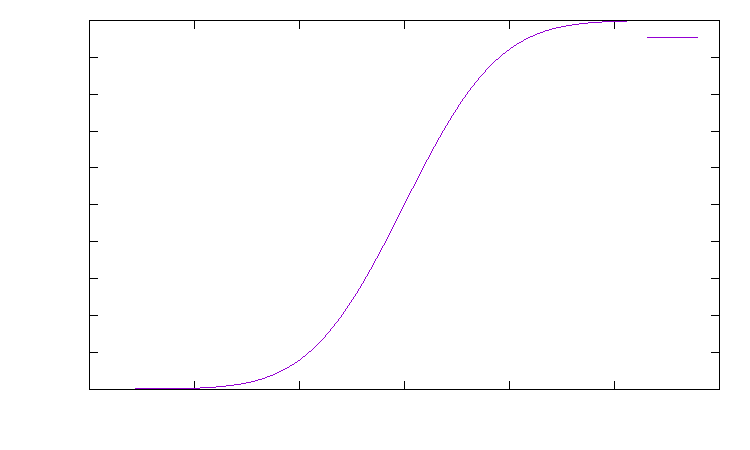
\includegraphics{plot-cairo}}%
    \gplfronttext
  \end{picture}%
\endgroup

\caption{ODE representation of the error function, erf(x).}
\label{fig:erf}
\end{figure}


\end{document}
